\section{Resultados y discusión}
\subsection{Comparación calculada, simulada y experimental}
La Tabla~\ref{tab:comparacion_integrada} aplica una misma metodología a las
cuatro configuraciones identificadas. C denota cálculo lineal, S la simulación
con ADC/DAC y E el experimento. En C se realimentan directamente los estados
verdaderos, por lo que esta columna es la referencia ideal de $A-BK$, no la
salida de otro estimador. El pico se busca en los primeros
\SI{100}{\milli\second} del transitorio; el valor final es la media de las
últimas 50 muestras. La matriz aumentada posee $\rho=0.8382$ en los cuatro
casos porque los polos de control son comunes y los polos del observador
permanecen desacoplados por el principio de separación.

\begin{table*}[t]
\centering
\caption{Comparación directa con el modelo identificado. Amplitudes, RMSE y
mando en mV; $t_p$ experimental en ms.}
\label{tab:comparacion_integrada}
\small
\resizebox{\textwidth}{!}{%
\begin{tabular}{@{}lrrrrrrrrrr@{}}
\toprule
Caso & Pico C & Pico S & Pico E & Final C & Final S & Final E & RMSE S--E & RMS $e_y$ E & $|u_{apl}|_{\max}$ E & $t_p$ E\\
\midrule
Predictor E1 & 58.01 & 62.55 & 65 & 50.00 & 61.66 & 46.12 & 13.35 & 2.91 & 77 & 40\\
Actual E1    & 58.01 & 61.66 & 65 & 50.00 & 61.66 & 49.62 & 12.15 & 2.29 & 92 & 18\\
Predictor E2 & 58.01 & 62.55 & 65 & 50.00 & 61.66 & 46.24 & 13.46 & 2.91 & 77 & 20\\
Actual E2    & 58.01 & 64.17 & 60 & 50.00 & 46.25 & 50.30 &  6.20 & 1.77 & 92 & 14\\
\bottomrule
\end{tabular}}
\end{table*}

La referencia ideal coincide en los cuatro casos: al desaparecer el error de
estimación, la dinámica restante es la de $A-BK$. La simulación no ideal
reproduce el crecimiento inicial, pero presenta niveles estacionarios
cuantizados. El experimento conserva la forma del transitorio y queda a uno o
pocos niveles del DAC/ADC alrededor de la referencia. En las condiciones
ensayadas, Actual E2 obtuvo la menor RMSE simulación--experimento y el menor
error observable RMS. La diferencia de régimen se asocia al efecto conjunto de
cuantización, ruido y calibración, no a una modificación de los polos de control.

\begin{figure*}[t]
\centering
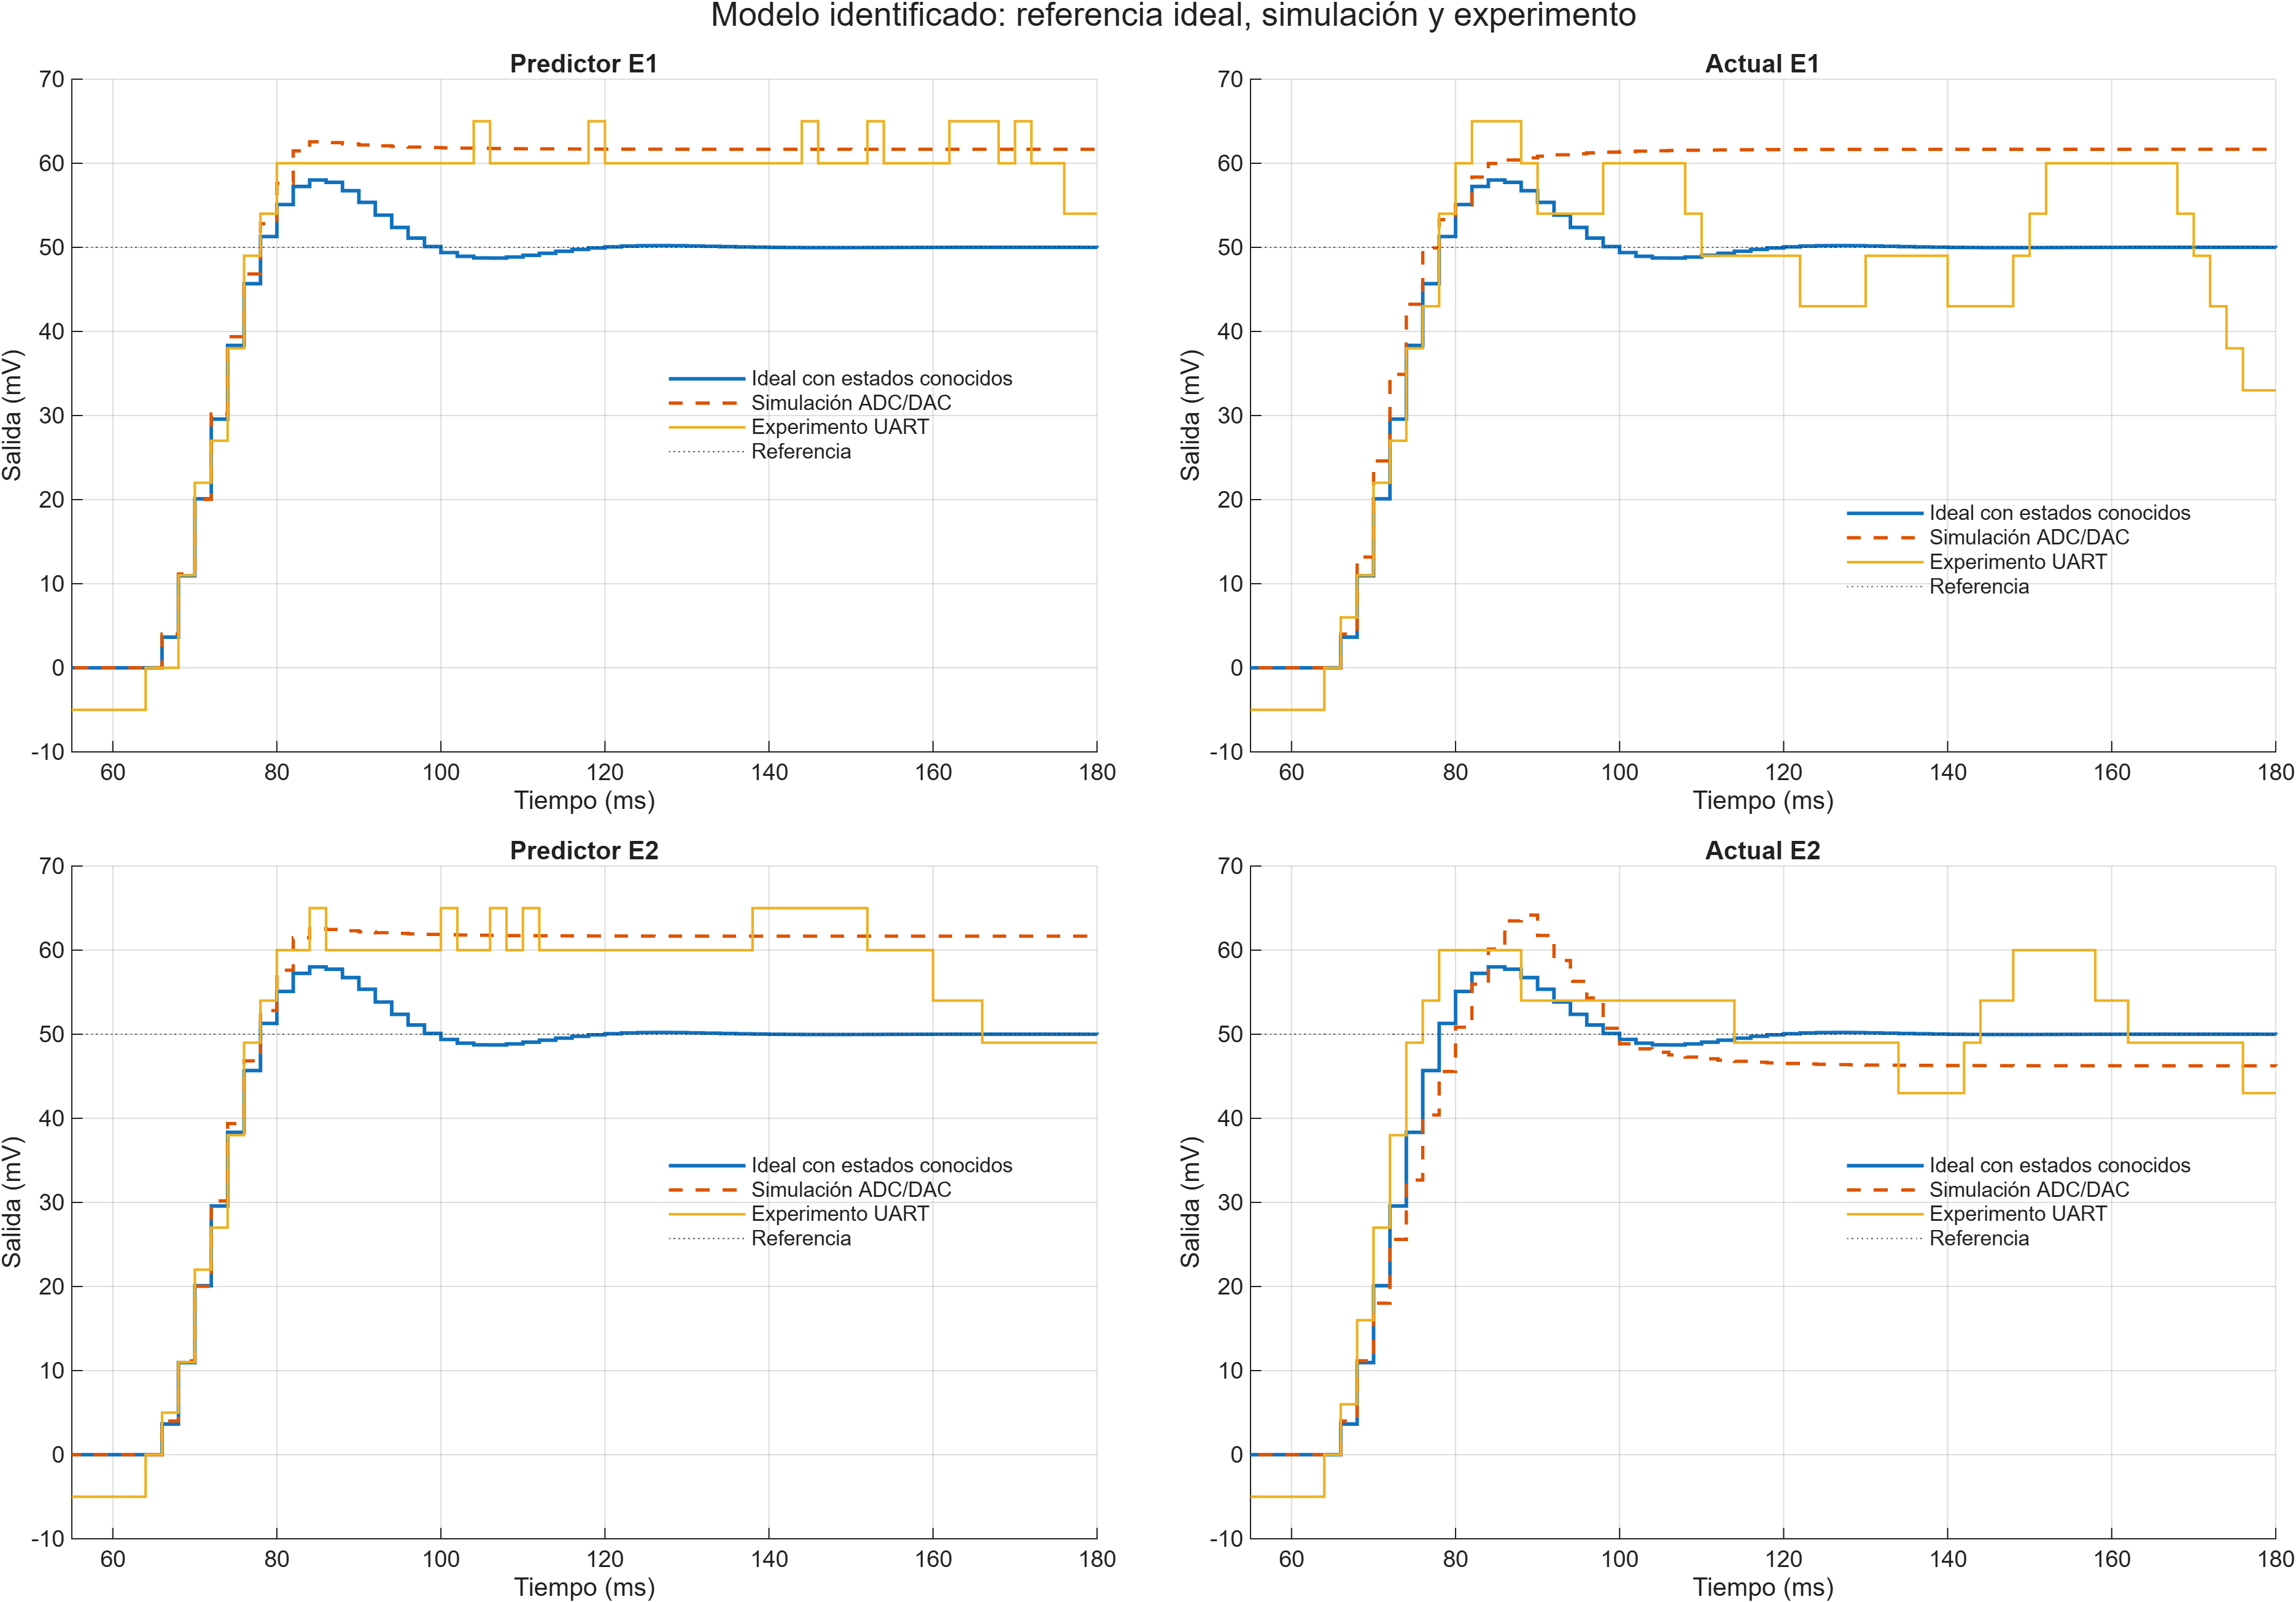
\includegraphics[width=\textwidth]{../05_Resultados/Validacion_Integrada_20261124/figuras/comparacion_calculada_simulada_experimental_4_casos.png}
\caption{Comparación de la referencia ideal con estados conocidos, la simulación
no ideal y la telemetría experimental para las cuatro configuraciones.}
\label{fig:comparacion_sim_exp}
\end{figure*}

La Tabla~\ref{tab:esfuerzo_ruido_tiempo} complementa los máximos con el valor
RMS del mando aplicado desde el escalón. La desviación estándar de $e_y$ usa
las últimas 50 muestras y separa la dispersión del sesgo. La fracción temporal
se define como $100t_{\mathrm{CPU,max}}/T_s$ y el margen como su complemento.

\begin{table}[t]
\centering
\caption{Esfuerzo, dispersión observable y margen temporal experimentales.}
\label{tab:esfuerzo_ruido_tiempo}
\small
\resizebox{\columnwidth}{!}{%
\begin{tabular}{@{}lrrrr@{}}
\toprule
Caso & $u_{\mathrm{RMS}}$ (mV) & $\sigma_{e_y}$ (mV) & CPU/$T_s$ (\%) & Margen (\%)\\
\midrule
Predictor E1 & 50,35 & 3,38 & 5,60 & 94,40\\
Actual E1    & 53,28 & 2,49 & 5,50 & 94,50\\
Predictor E2 & 49,78 & 3,49 & 5,55 & 94,45\\
Actual E2    & 51,03 & 1,72 & 5,55 & 94,45\\
\bottomrule
\end{tabular}}
\end{table}

Actual E2 presentó la menor dispersión de $e_y$ en esta campaña. Este resultado
se limita a una ejecución por caso y no se generaliza como una propiedad
universal frente al ruido. Los cuatro valores de $u_{\mathrm{RMS}}$ fueron
similares y el cálculo ocupó como máximo el 5,60\,\% de $T_s$.

\subsection{Estados estimados y errores en las cuatro configuraciones}
La Fig.~\ref{fig:estados_estimados} presenta $\hat x_1$, $\hat x_2$ y la salida
medida. $\hat x_1$ es un estado interno de la realización identificada; sus
valores negativos no representan una tensión medida directamente. La
Fig.~\ref{fig:errores_estimacion} muestra el error observable
$e_y=y-\hat x_2$. Desde el escalón, los RMS fueron 2,91; 2,29; 2,91 y
\SI{1.77}{\milli\volt} para Predictor E1, Actual E1, Predictor E2 y Actual E2.
En ambas familias el estimador actual redujo el RMS respecto del predictor,
coherente con el uso de la muestra presente antes de calcular el mando.

\begin{figure*}[t]
\centering
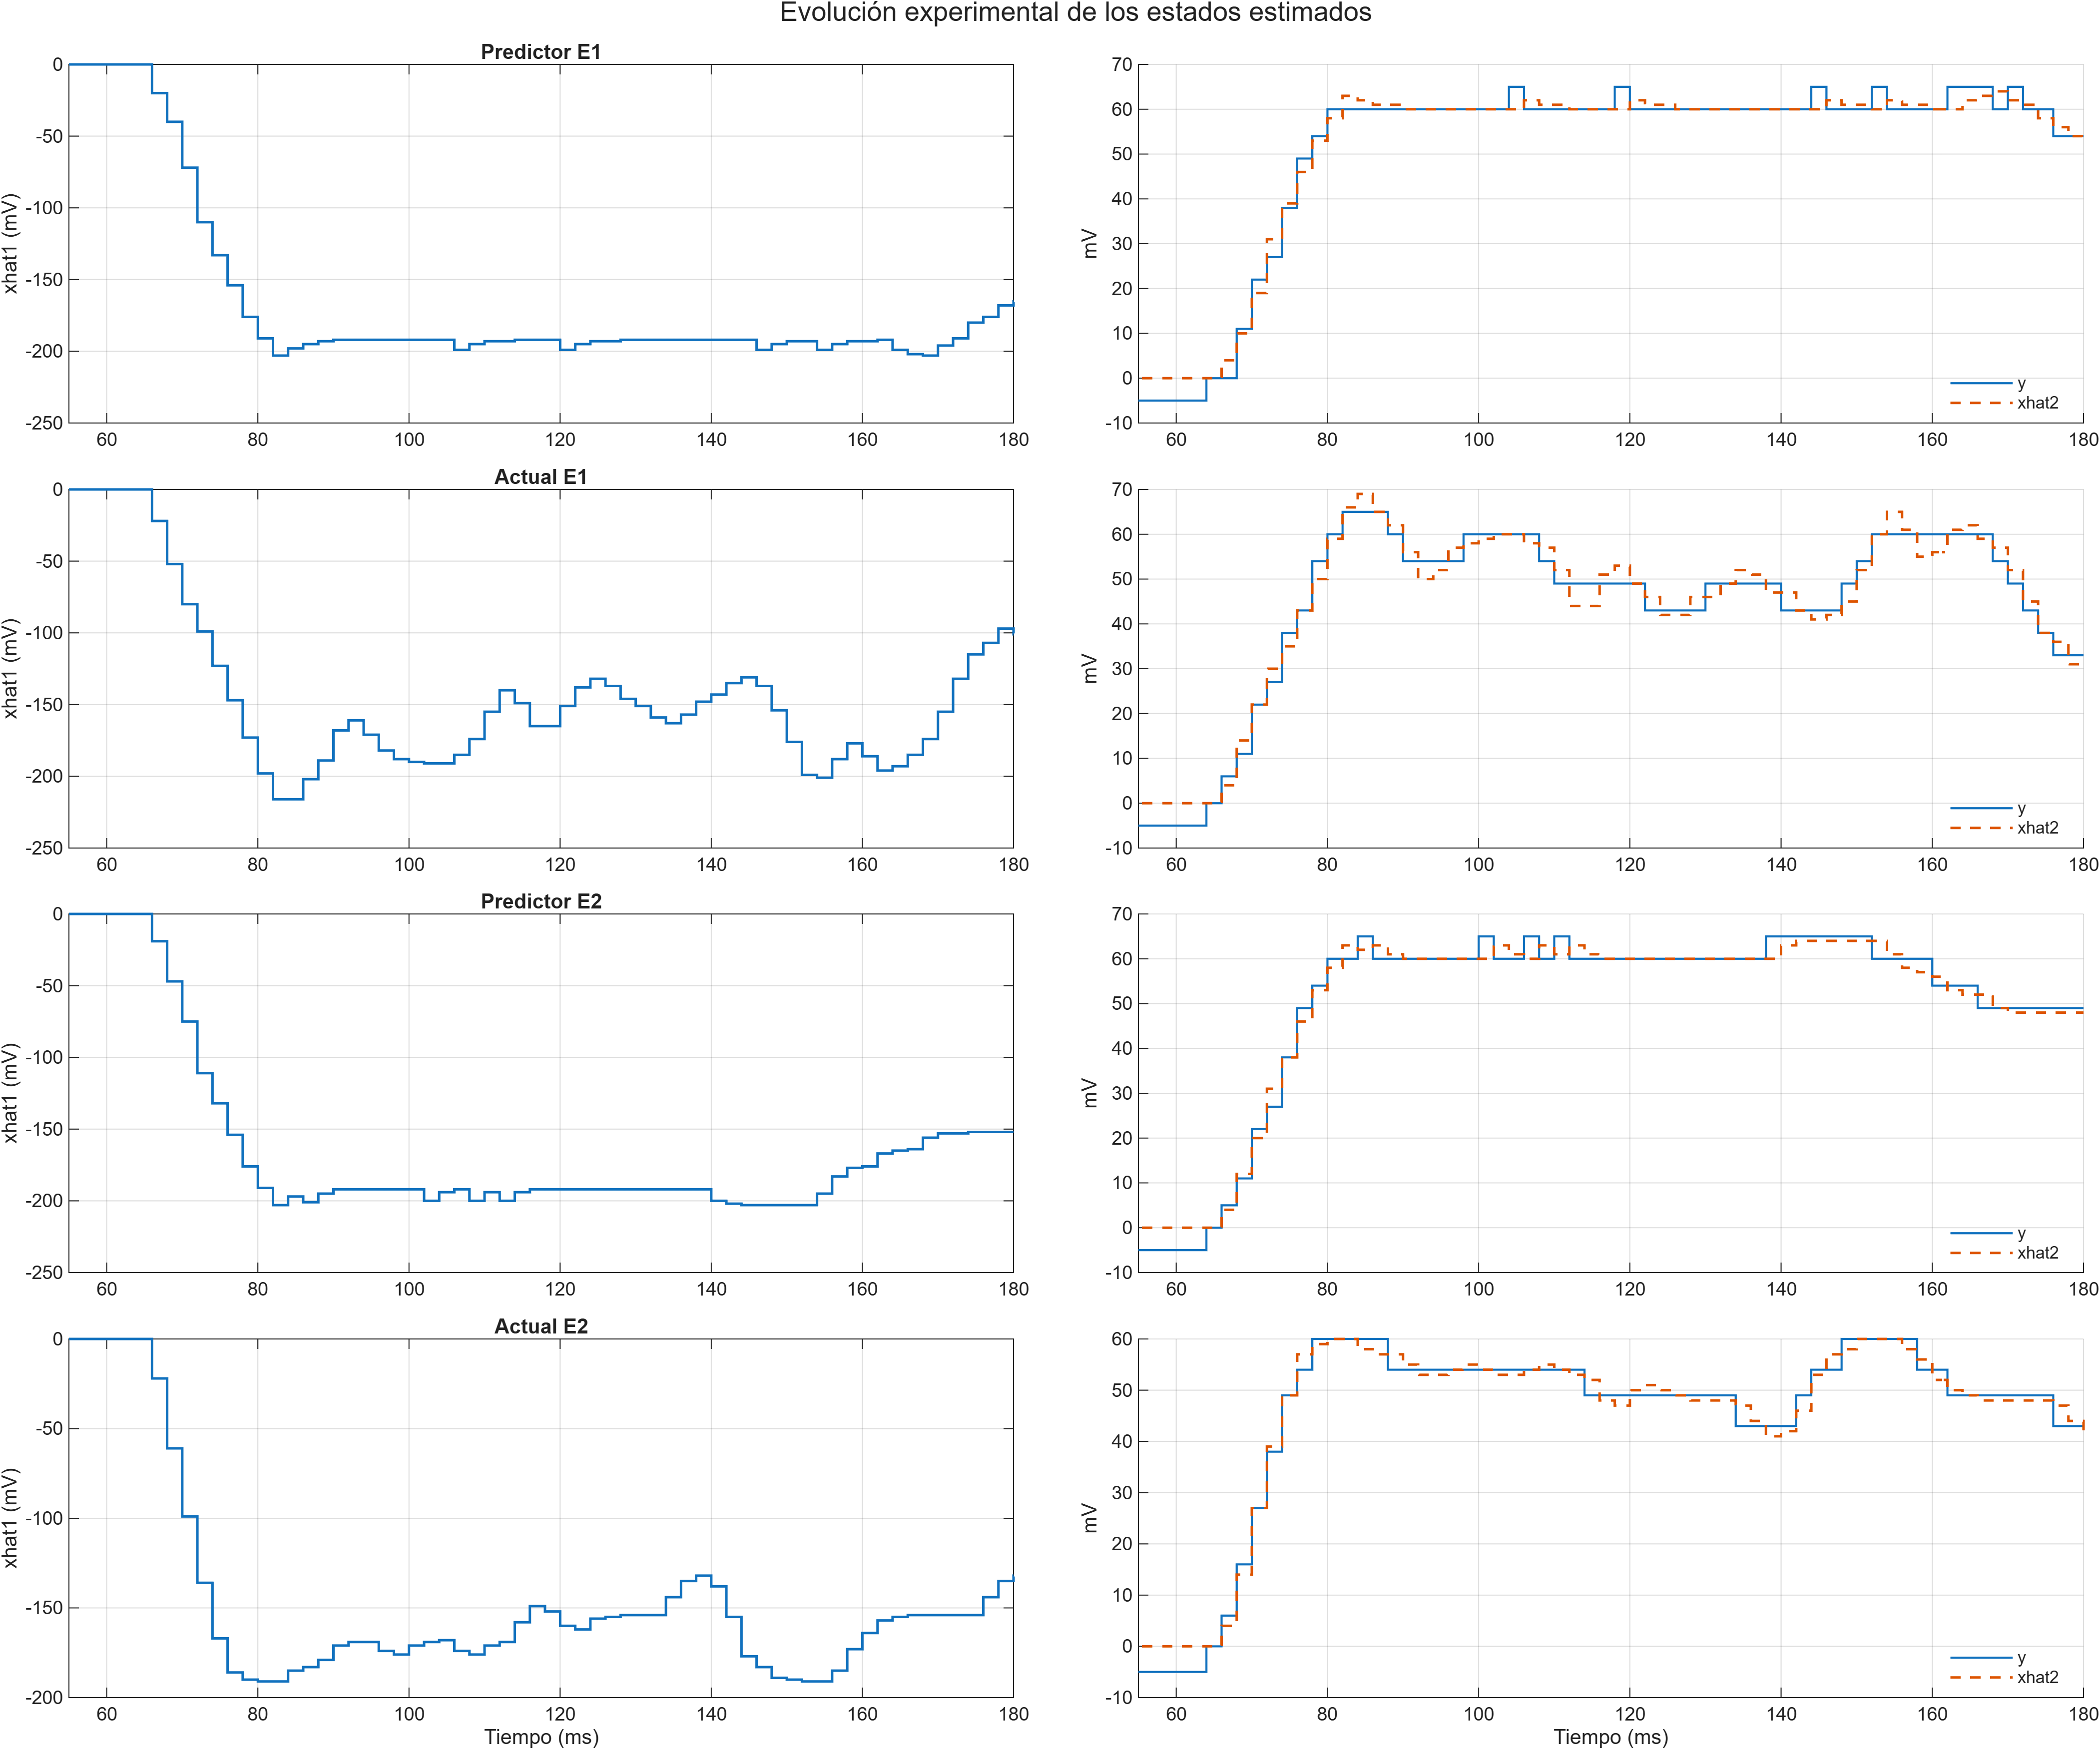
\includegraphics[width=\textwidth]{../05_Resultados/Validacion_Integrada_20261124/figuras/estados_estimados_experimentales_4_casos.png}
\caption{Evolución experimental de los estados estimados. La salida medida se
superpone con $\hat x_2$; $\hat x_1$ no posee medición independiente.}
\label{fig:estados_estimados}
\end{figure*}

\begin{figure*}[t]
\centering
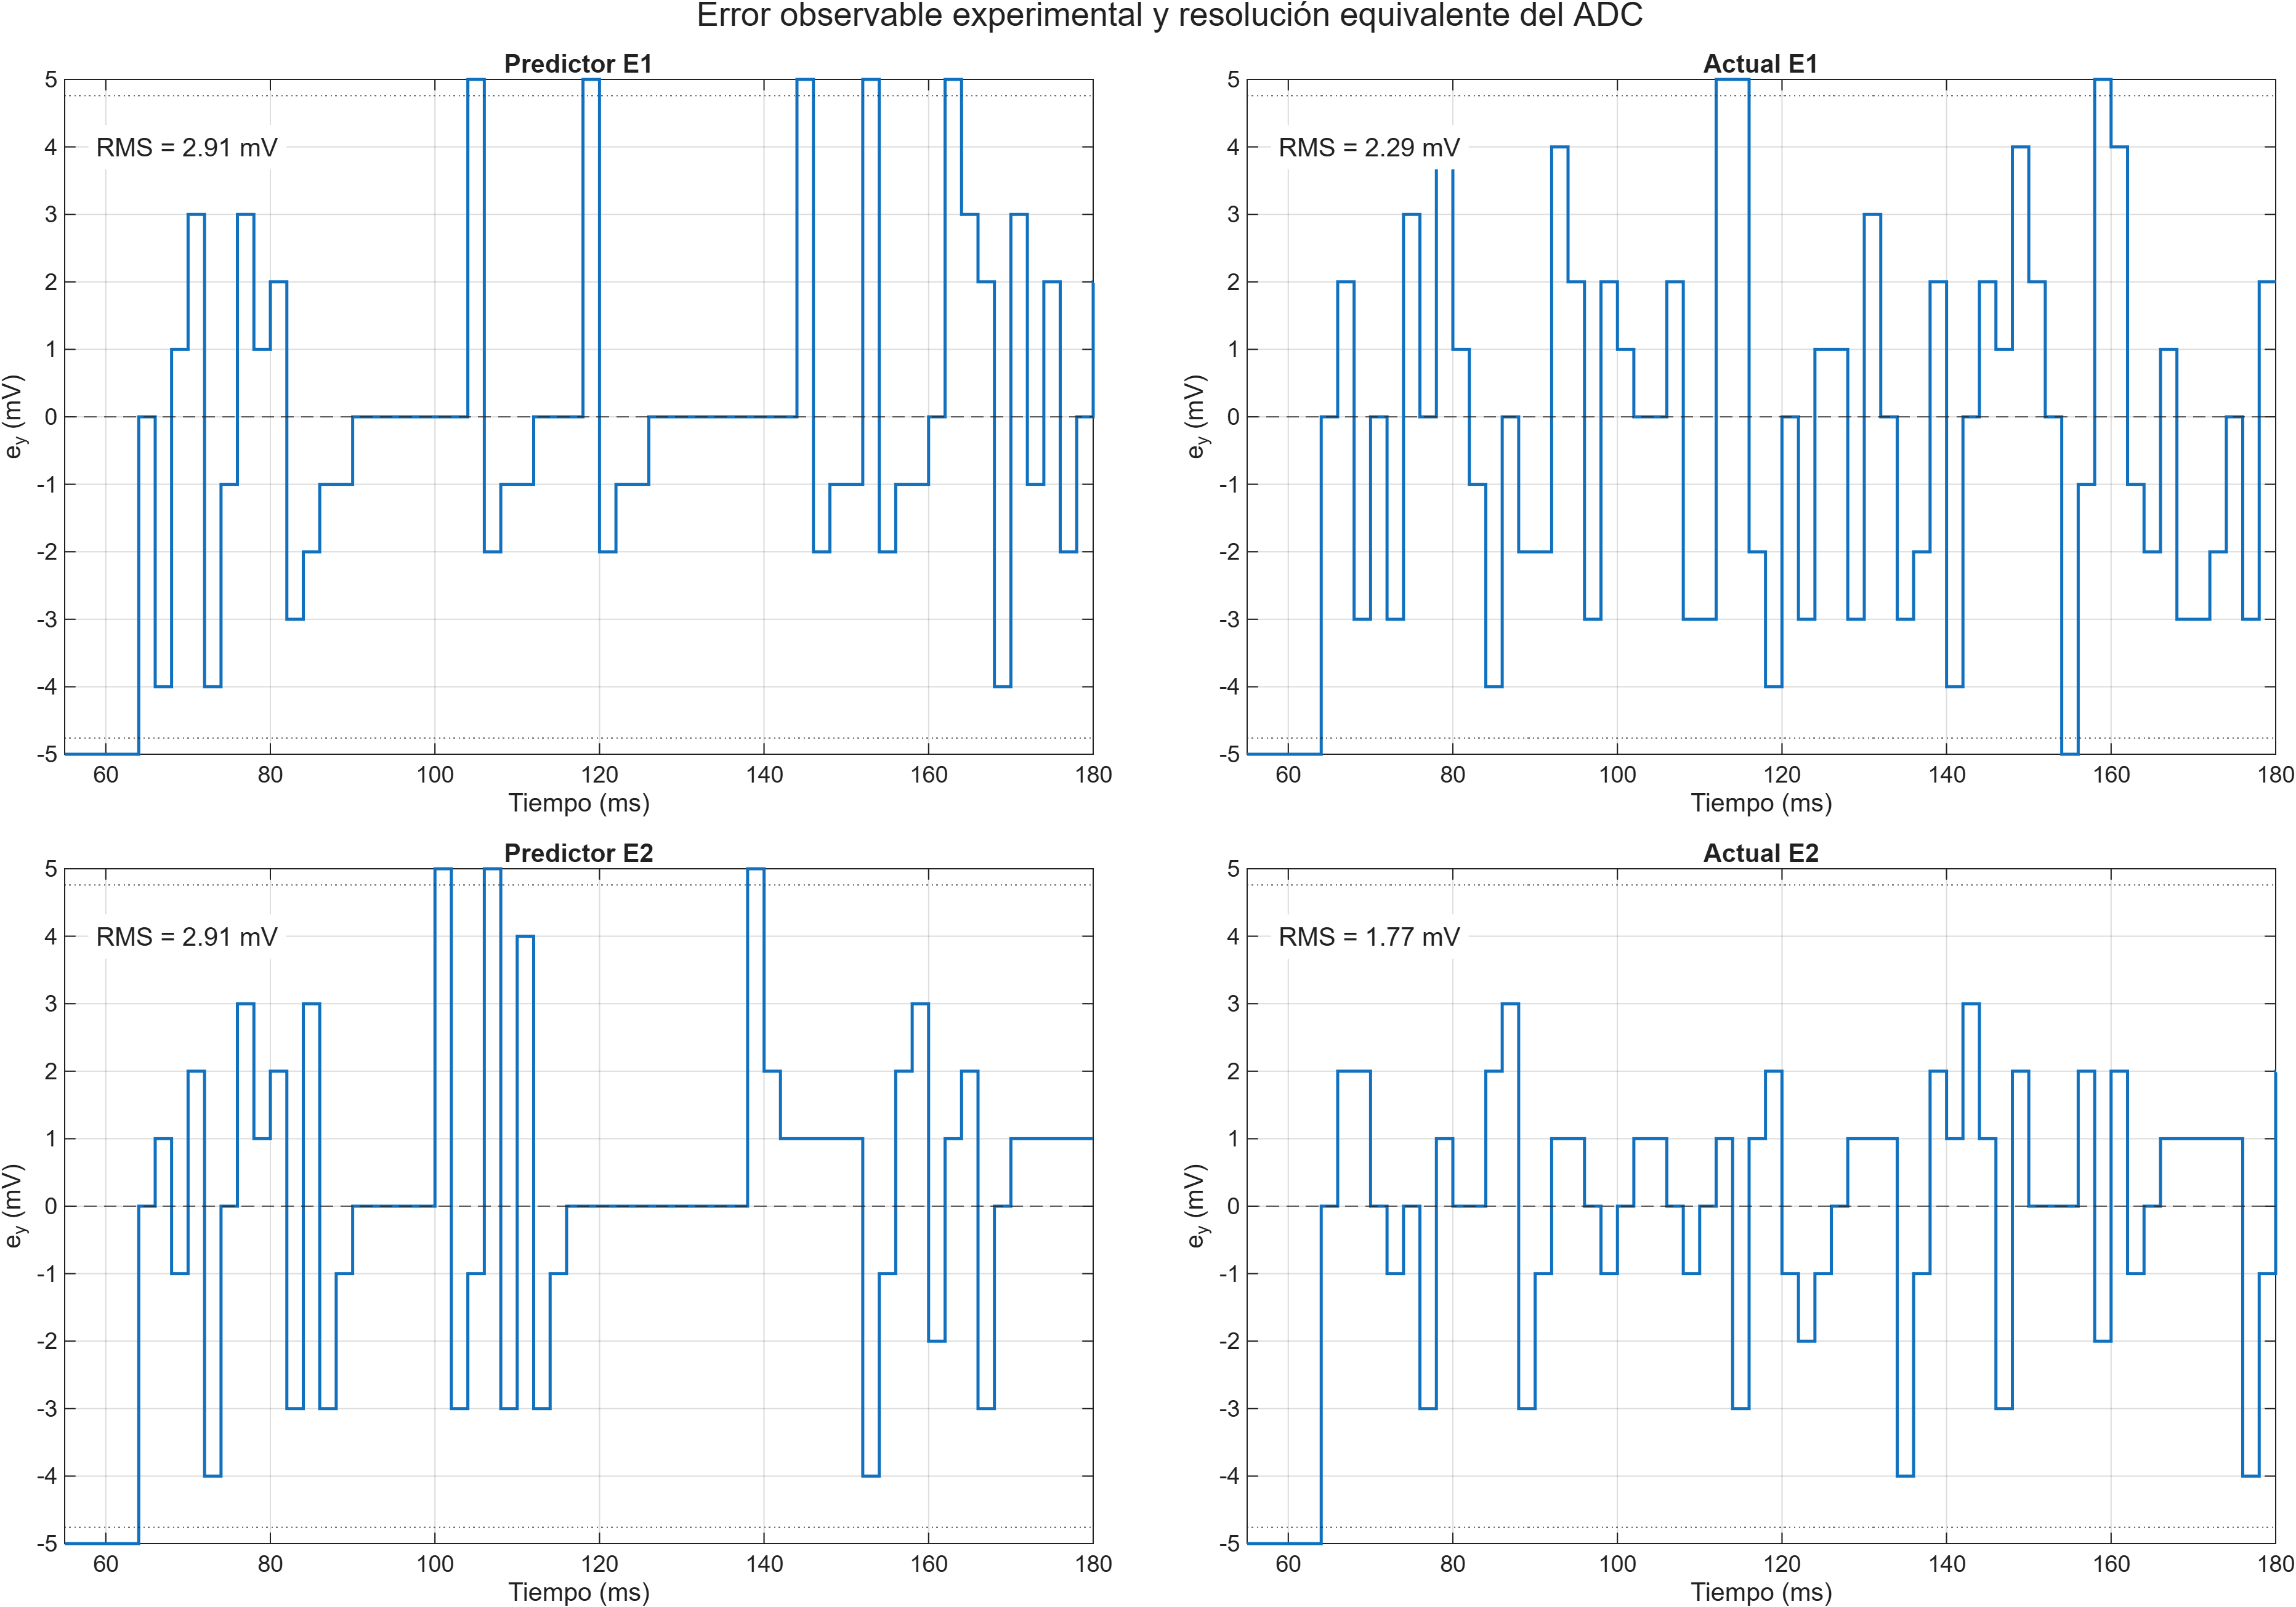
\includegraphics[width=\textwidth]{../05_Resultados/Validacion_Integrada_20261124/figuras/errores_estimacion_experimentales_4_casos.png}
\caption{Error observable experimental. Las líneas punteadas indican la
resolución equivalente aproximada de una cuenta ADC (\SI{4.76}{\milli\volt}).}
\label{fig:errores_estimacion}
\end{figure*}

\subsection{Rapidez de convergencia y efecto de la muestra presente}
Se emplearon dos indicadores distintos. Para los polos del observador se calculó
\begin{equation}
N_{2\%}=\left\lceil\frac{\log(0.02)}{\log\rho_o}\right\rceil,
\qquad t_{2\%}=N_{2\%}T_s,
\end{equation}
donde $\rho_o$ es el mayor módulo de los polos asignados. En la simulación de
la perturbación se definió $t_c$ como el primer instante a partir del cual
$\|e[k]\|_2<10^{-4}$ V se cumple para todas las muestras restantes. Por tanto,
$t_{2\%}$ y $t_c$ son referencias complementarias y no métricas idénticas.

\begin{table}[t]
\centering
\caption{Convergencia teórica y simulada del error de estimación.}
\label{tab:convergencia_teorica}
\small
\resizebox{\columnwidth}{!}{%
\begin{tabular}{@{}lrrrrr@{}}
\toprule
Familia & $\rho_o$ & $N_{2\%}$ & $t_{2\%}$ (ms) & $t_c$ Pred. (ms) & $t_c$ Actual (ms)\\
\midrule
E1, $0.25\pm j0.05$ & 0,25495 & 3 & 6 & 6 & 6\\
E2, $0.20\pm j0.10$ & 0,22361 & 3 & 6 & 8 & 8\\
\bottomrule
\end{tabular}}
\end{table}

Para aislar el transitorio de estimación se simuló
$\hat x[0]-x[0]=[0.02\;-0.01]^T$ V. Predictor y actual alcanzaron
persistentemente $\|e\|_2<10^{-4}$ en 6 ms para E1 y en 8 ms para E2. La
ventaja del estimador actual aparece inmediatamente después de incorporar
$y[k]$: el error inicial corregido fue 11,69 mV frente a 22,36 mV en E1, y
8,37 mV frente a 22,36 mV en E2. Aunque el cálculo modal redondea ambas familias
a tres muestras, el cruce de un umbral absoluto depende también de la dirección
del error inicial y de la combinación modal; la tasa asintótica queda determinada
por los polos asignados.
Una vez extinguido ese error, las cuatro curvas de salida obedecen a $A-BK$.

\begin{figure*}[t]
\centering
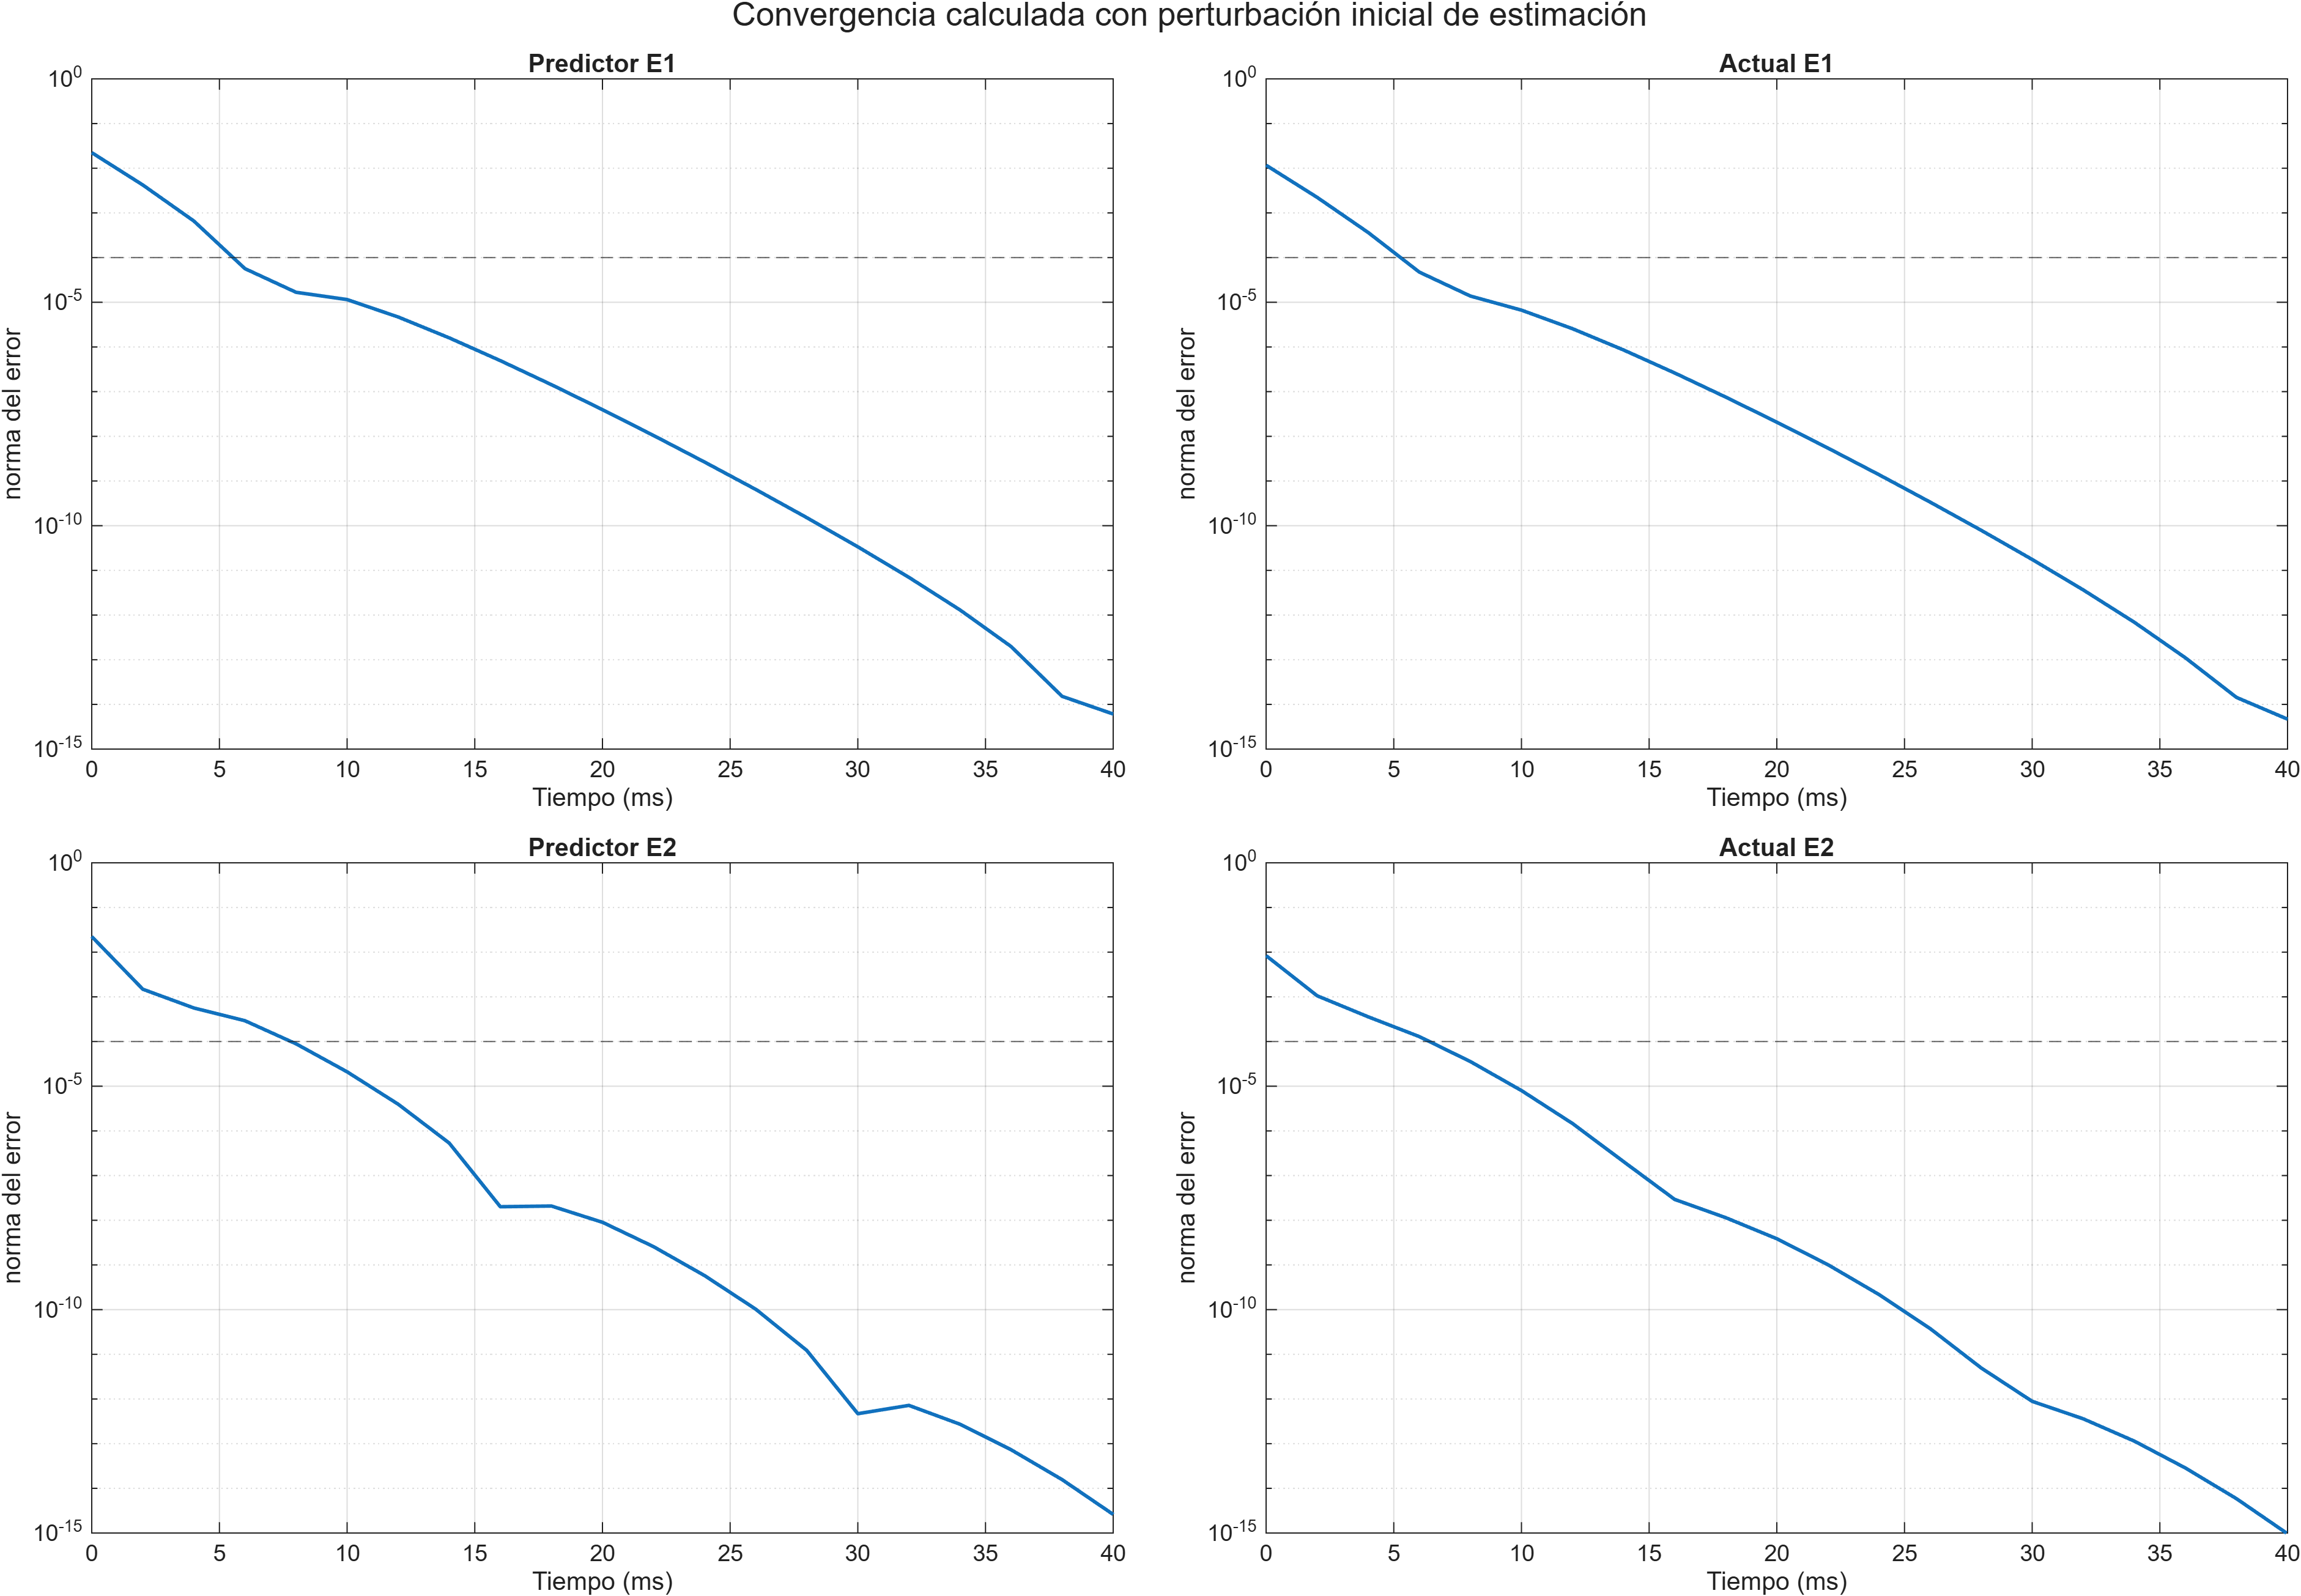
\includegraphics[width=\textwidth]{../05_Resultados/Validacion_Integrada_20261124/figuras/convergencia_rediseno_identificado_4_casos.png}
\caption{Convergencia calculada del error de estado ante la misma perturbación
inicial, con escala vertical común.}
\label{fig:convergencia_identificada}
\end{figure*}

\subsection{Validación física simultánea}
El Rigol confirmó que J5 y J7 cambiaron simultáneamente al terminar cada
ensayo. La Tabla~\ref{tab:rigol} usa las medianas del primer y último 20\,\% de
cada registro para evitar que el ruido de alta frecuencia sesgue la amplitud.
Las razones $\Delta J7/\Delta J5$ permanecieron entre 0,974 y 1,064.

\begin{table}[t]
\centering
\caption{Variaciones físicas medidas por el Rigol.}
\label{tab:rigol}
\small
\begin{tabular}{@{}lrrr@{}}
\toprule
Caso & $\Delta J5$ (mV) & $\Delta J7$ (mV) & Razón\\
\midrule
Predictor E1 & 44 & 46,0 & 1,046\\
Actual E1    & 50 & 53,2 & 1,064\\
Predictor E2 & 46 & 44,8 & 0,974\\
Actual E2    & 48 & 50,0 & 1,042\\
\bottomrule
\end{tabular}
\end{table}

\begin{figure*}[t]
\centering
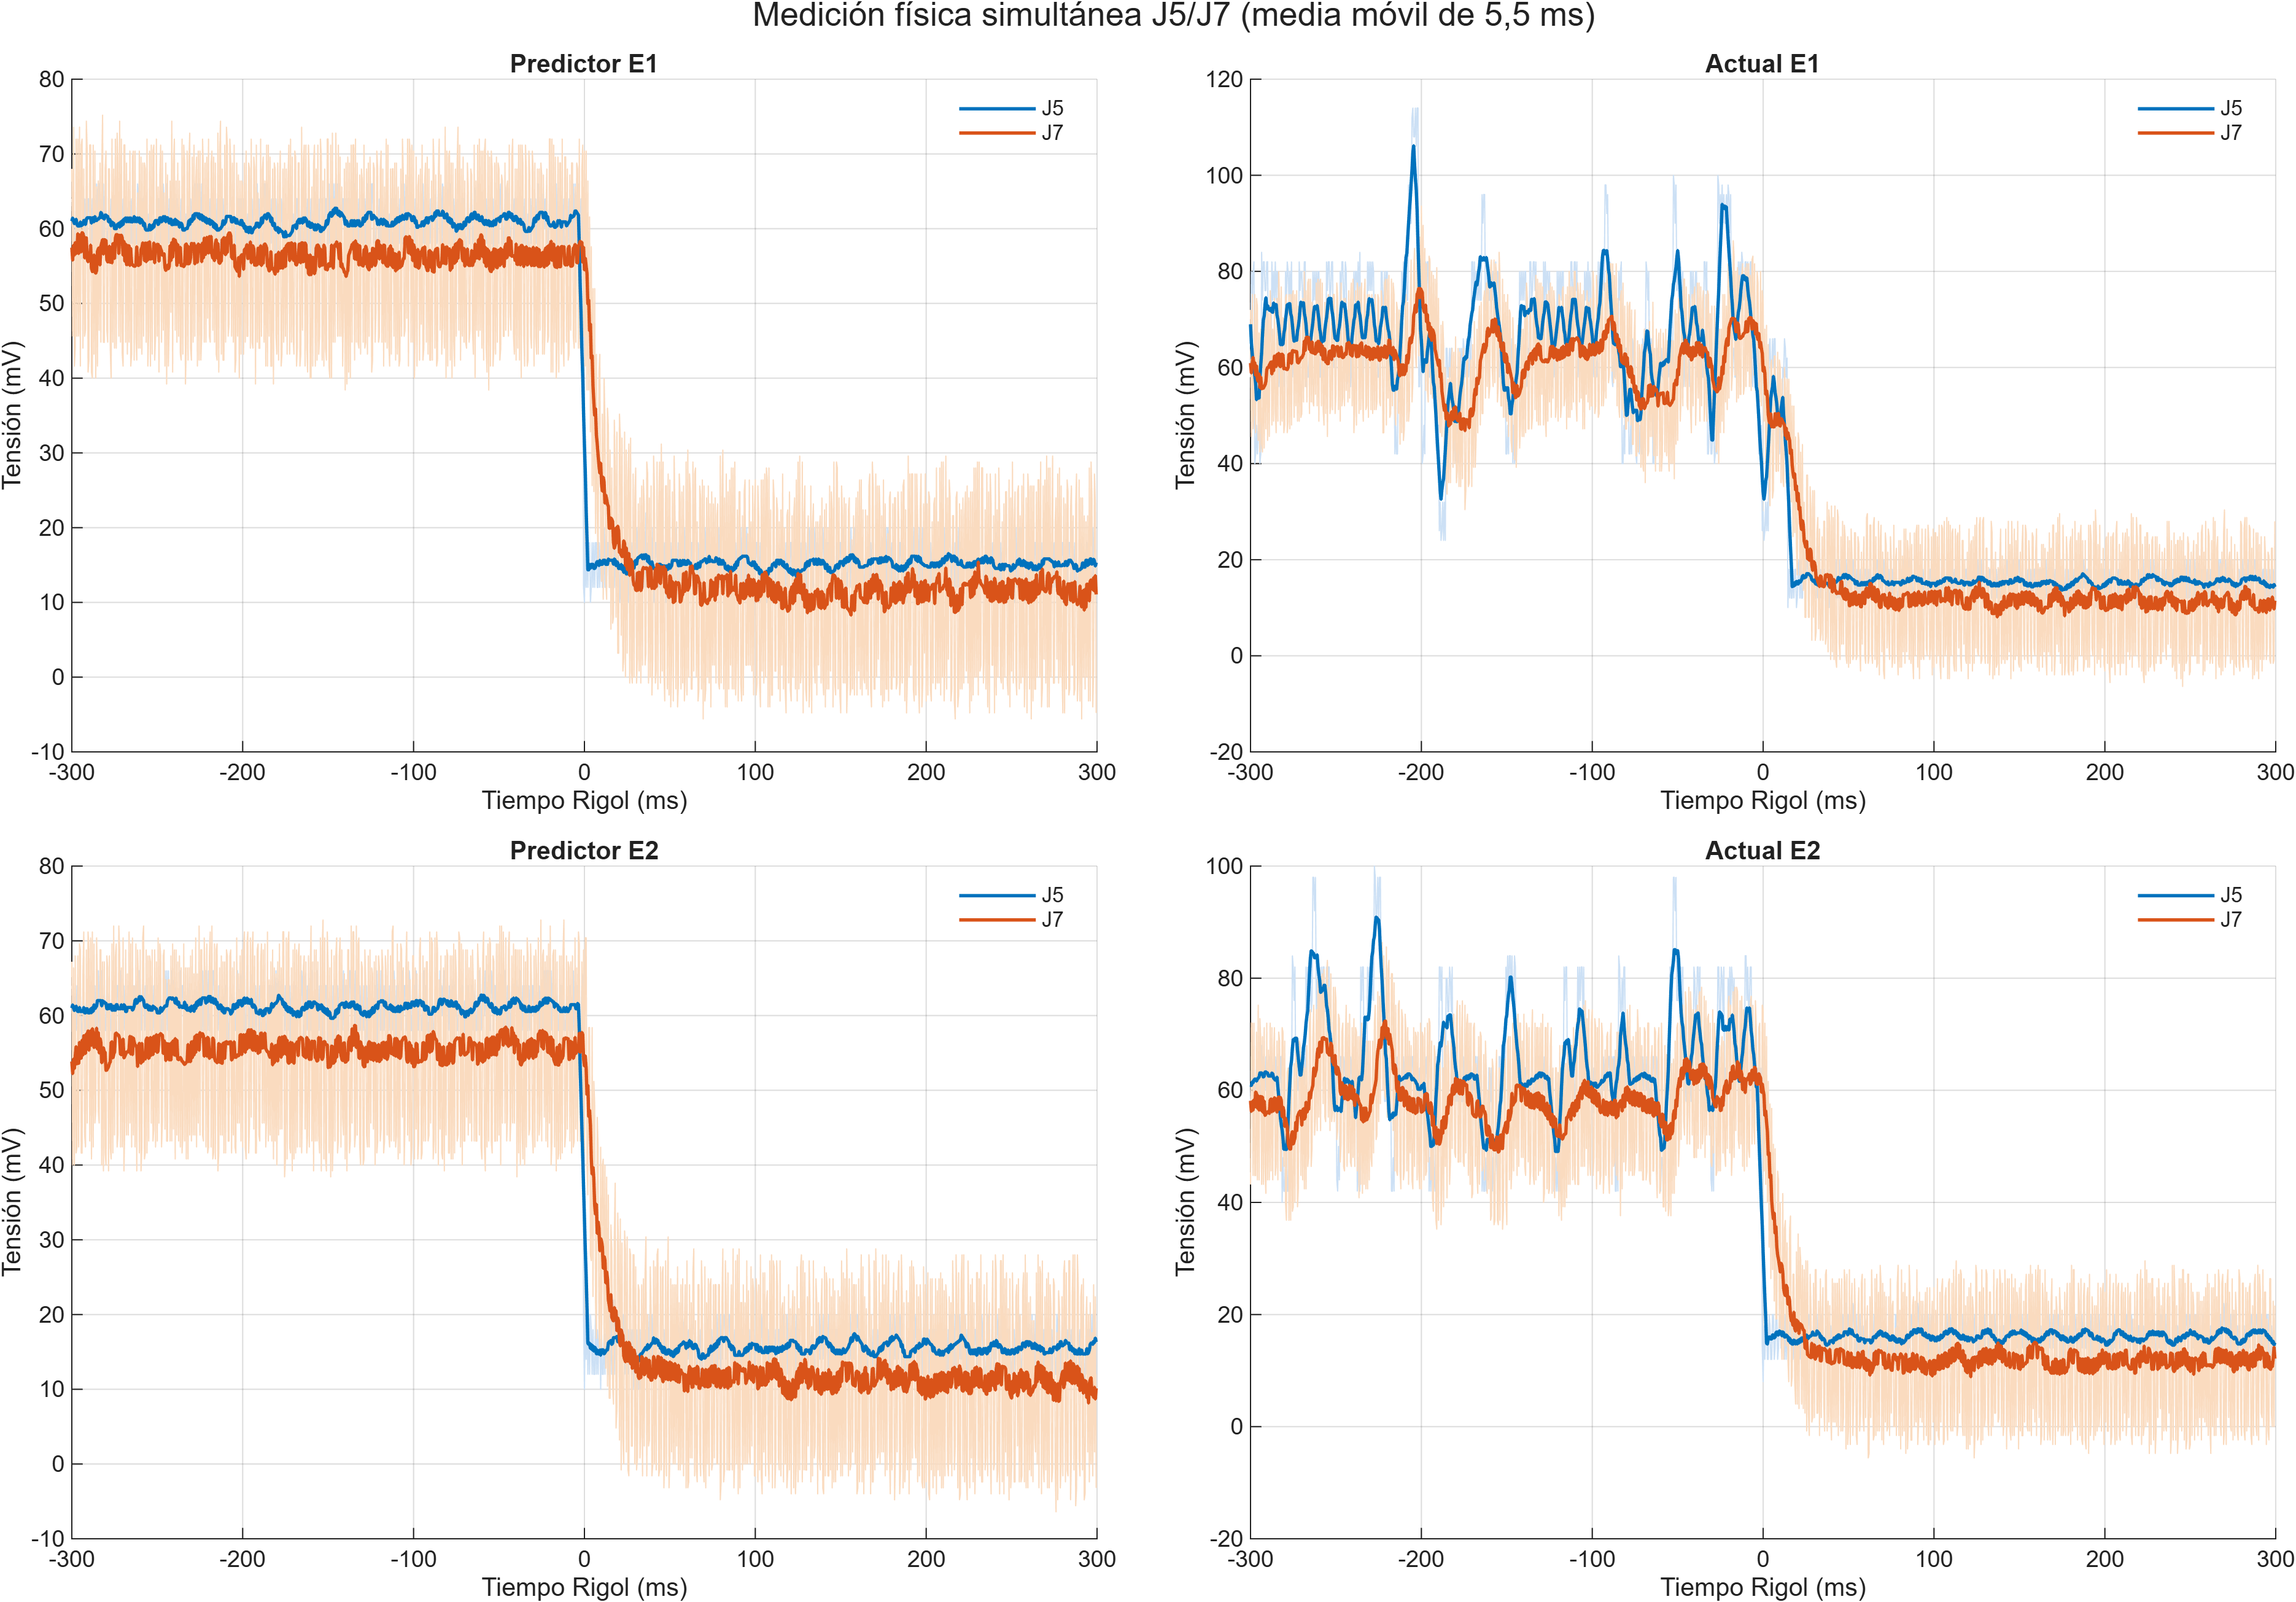
\includegraphics[width=\textwidth]{../05_Resultados/Validacion_Integrada_20261124/figuras/mediciones_fisicas_Rigol_4_casos.png}
\caption{Ondas J5/J7 al retorno seguro. Las líneas intensas muestran una media
móvil de 5,5 ms; los datos crudos se preservan en segundo plano.}
\label{fig:rigol_fisico}
\end{figure*}

\subsection{Resolución del actuador}
La Tabla~\ref{tab:cuantizacion} compara predictor y actual por índice de muestra
dentro de cada familia. ``Compresión'' es la fracción de solicitudes diferentes
que terminó en el mismo nivel del DAC. Aun cuando los mandos calculados difieren,
una proporción importante se convierte en el mismo valor físico.

\begin{table}[t]
\centering
\caption{Coincidencia de acciones por cuantización del DAC.}
\label{tab:cuantizacion}
\small
\begin{tabular}{@{}lrrr@{}}
\toprule
Par & Mismo DAC & Solicitud distinta, mismo DAC & Compresión\\
\midrule
E1 & 46,48\,\% & 32,42\,\% & 37,73\,\%\\
E2 & 61,33\,\% & 45,70\,\% & 54,17\,\%\\
\bottomrule
\end{tabular}
\end{table}

Los pasos nominales fueron \SI{15.37}{\milli\volt} en la rama positiva y
\SI{10.56}{\milli\volt} en la negativa. Las diferencias solicitadas medias
entre arquitecturas fueron 9,44 mV para E1 y 6,34 mV para E2, magnitudes del
orden de un paso. Con una referencia de solo \SI{50}{\milli\volt}, esta
resolución reduce la capacidad de distinguir estructuras a partir de la salida.

\subsection{Verificación temporal y alcance experimental}
Cada captura contiene 256 muestras, mediana de
\SI{2000}{\micro\second}, tiempo máximo de CPU entre 110 y
\SI{112}{\micro\second}, cero banderas y disparo físico sin forzado. Los
metadatos registran el modelo, la arquitectura y la ubicación de polos de cada
ensayo. El peor caso ocupó 5,60\,\% del período y dejó 94,40\,\% de
margen, por lo que el retardo de cómputo no fue comparable con $T_s$. Por tanto,
la actualización del DAC se completó con holgura dentro de cada período.

La comparación experimental corresponde a una ejecución por configuración con
una referencia de \SI{50}{\milli\volt}. Como $x_1$ no dispone de una medición
independiente, su error se analiza en simulación; en el banco se utiliza
$e_y=y-\hat x_2$. La UART registra el transitorio completo y el osciloscopio
corrobora la amplitud física y la simultaneidad de J5 y J7. Los CSV crudos, las
métricas y el script se conservan para reproducir el análisis.
